\chapter{Fundamentação Teórica}
\label{ch:fundamentacao}
\par Neste capítulo ser\~ao fundamentados os conhecimentos b\'asicos para o entendimento do trabalho.

\section{Java}

\par Java é uma linguagem de programação multiplataforma, concorrente (executa mais de uma tarefa em paralelo), baseada em classes e orientada a objetos \cite{joy2000java}.
\par A linguagem Java é compilada e interpretada. Após escrever um programa em Java, estes são salvos como código fonte com extensão ".java". Quando estes códigos fontes são compilados, um arquivo binário chamado de arquivo de classe com extensão ".class" é gerado. Estes arquivos não são executados diretamente pelos processadores, pois eles não contêm instruções para os mesmos. Os programas Java são compilados em um formato de arquivo chamado \textit{bytecode}. Desta forma, esses programas podem ser executados em qualquer sistema operacional que possua um interpretador JVM (Java \textit{Virtual Machine}) em um JRE (Java \textit{Runtime} \textit{Environment}) conforme Figura \ref{fig:ambiente java}. Assim, o código precisa ser compilado apenas uma vez em cada sistema para funcionar, pois os \textit{bytecodes} serão executados da mesma forma em qualquer plataforma \cite{arnold2005java}.

\begin{figure}[H]
    \centering
    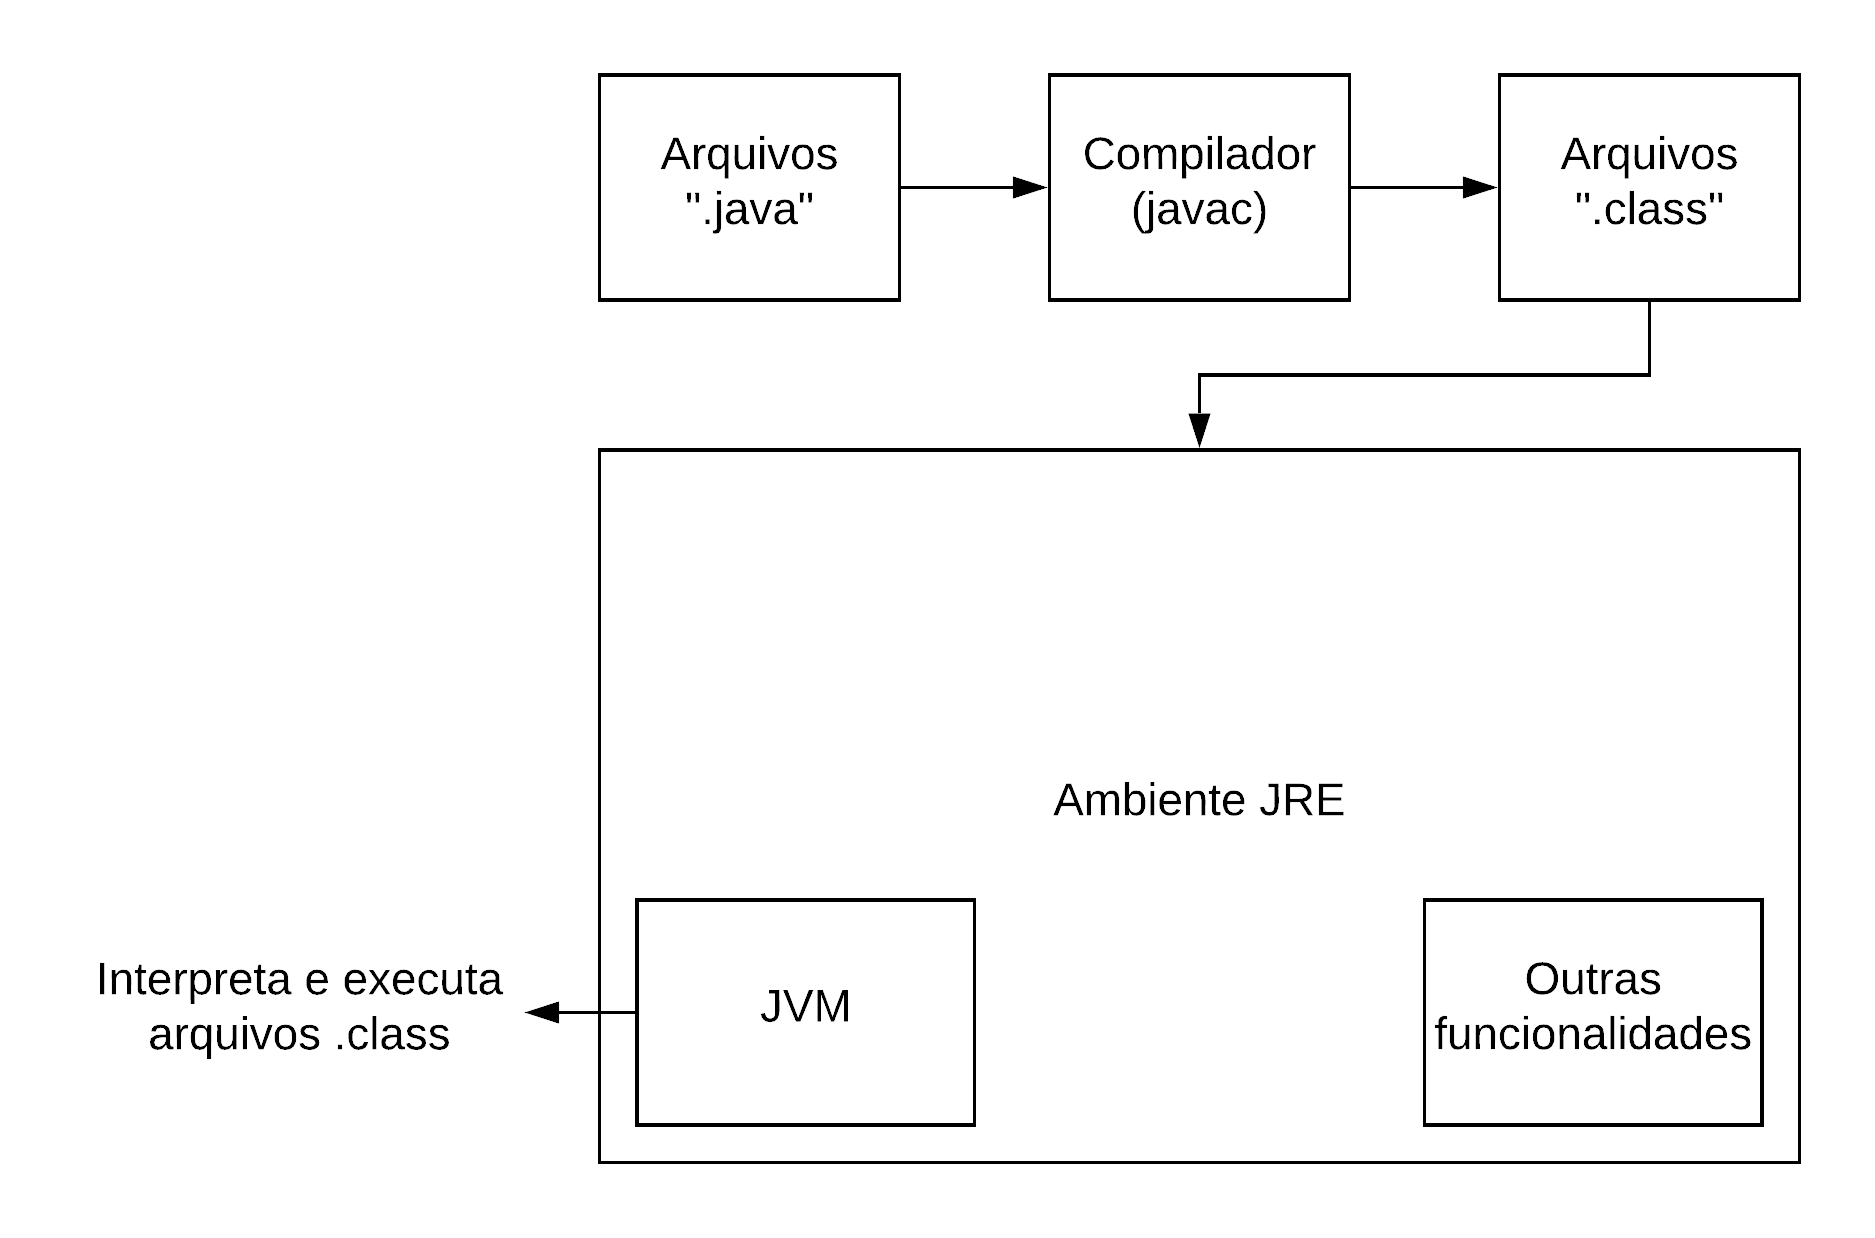
\includegraphics[scale=0.2]{src/imagens/cap1/ambiente-java.png}
    \caption{Ambiente Java}
    \label{fig:ambiente java}
    \fonte{Adaptado de \citeonline{introductionToTheJavaProgrammingEnvironment}}
\end{figure}

\par É uma linguagem fortemente tipada, isto é, as características das variáveis tem que ser definidas em tempo de compilação. Ela possui um coletor de lixo (\textit{garbage collector}) para evitar problemas de segurança como \textit{deadlock}. \cite{joy2000java}

\subsection{Reflexão}

% Magão usa \citeonline{guerra2014componentes} By: Menino
% agradecer o menino depois
\par De acordo com \citeonline{guerra2014componentes} o conceito de reflexão pode ser definido como um processo em que um programa pode visualizar e alterar sua própria estrutura assim como seu comportamento. As classes de reflexão disponíveis na linguagem de programação Java, se localizam no pacote \textit{java.lang.reflect}. Existem classes localizadas neste pacote que não aplicam o conceito de reflexão, mas sim o de introspecção, que é a obtenção de informações sobre classes, sem a modificação da estrutura das mesmas.

\subsection{Anotação}

\par Anotações em Java, são utilizadas para definição de metadados, isto é, informações sobre algo, e podem ser inseridas em: Pacotes, classes, interfaces, métodos, declaração de variáveis, construtores e em anotações. Por padrão, nenhum comportamento é alterado com a adição de uma anotação, isto é feito a partir de métodos que verificam a existência das mesmas \cite{bloch2004jsr}.

\section{Framework}

\par Um framework pode ser considerado um software incompleto que é especializado com o comportamento de uma aplicação externa \cite{johnson1988designing}. Este determina a arquitetura que a aplicação utilizará, sua organização, como: convenções de nomes, arquivos externos de configuração e/ou anotações. Isto é definido para que o desenvolvedor tenha que se preocupar apenas com o projeto que está trabalhando. A forma que o framework realiza esta organização deve ser baseada no que é mais viável para solucionar esta situação comum em relação ao problema encontrado, permitindo que a tarefa repetitiva ou específica seja reaproveitada em novos projetos.
Baseado nisso frameworks permitem que aplicações com estruturas semelhantes sejam criadas, facilitando a manutenção, padronização e legibilidade do código, entretanto, isto restringe o desenvolvedor a solução que o framework aplica, não permitindo que o desenvolvedor siga por determinados caminhos ou tome certas decisões no projeto.\cite{gamma2009padroes}

\subsection{Frameworks horizontais}

\subsection{Frameworks verticais}

\section{Gamification}
%falar sobre funções executivas talvez seja interessante
\par Gamification é a utilização de conceitos de jogos, sendo eles: Ganho de pontos, \textit{ranking}, troféus, \textit{rewards}, em aplicações com outros contextos. \textit{Softwares} de e-commerce, sites de e-learning, são alguns exemplos de contextos onde o gamification pode ser aplicado, o propósito do gamification é fazer com que a utilização das aplicações não diminua com o tempo, proporcionando melhor experiência ao usuário, pois as conquistas adquiridas durante a utilização contribuem nesta tarefa. Um exemplo de aplicação que utiliza gamification é a foldit \cite{burke2012behind}, que utiliza conceitos de pontos e troféus em um jogo de quebra cabeça, para na verdade, prever a estrutura da proteína humana \cite{deterding2011gamification}.

\section{Esfinge Project}

\par Esfinge Project\footnote{O projeto está disponível no endereço: http://esfinge.sf.net} é um projeto \textit{open-source} iniciado em 2011 por Dr. Eduardo Guerra junto a GSW, que tem como objetivo a criação de soluções reutilizáveis para um desenvolvimento ágil, um produto final flexível e de fácil manutenção.
\par O projeto disponibiliza 9 frameworks até o momento, estes são: QueryBuilder, Comparison, Guardian, AOM Role Mapper, SystemGlue, Gamification, Metadata, Classmock, ReTest.
\par Todos os frameworks citados acima seguem uma filosofia que consiste em: Configuração de metadados para que o comportamento desejado ocorra; Componentes que podem ser integrados a aplicações de forma simples; Pontos de extensão para criação de novas funcionalidades; Remover a preocupação com a solução que o framework disponibiliza, permitindo que o desenvolvedor foque apenas em sua aplicação específica \cite{esfinge2011}.

\subsection{Esfinge Gamification}

\par O Esfinge Gamification é um \textit{framework} que aplica lógica gamification, para \textit{softwares} que necessitam destes processos. Independente do domínio do \textit{software} é possível utilizar o \textit{framework}, pois este é desacoplado de lógicas da aplicação, sua responsabilidade é a tratativa dos dados de gamificação, portanto, pode ser integrado a qualquer programa Java, permitindo que o desenvolvedor foque na solução que está trabalhando, e deixe as responsabilidades de gamificação para o \textit{framework}  \cite{esfinge2011}.
\par O comportamento do framework é especificado via metadados, estes são anotações que podem ser inseridas nos métodos do software. Existem quatro tipos de processos implementados pelo \textit{framework}, estas são: Ponto, Ranking, \textit{Reward}, Troféu vide Figura \ref{fig:arquitetura-esfinge-gamification}. 

\begin{figure}[H]
    \centering
    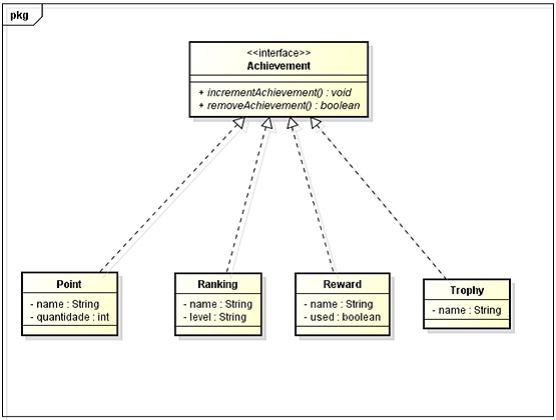
\includegraphics{src/imagens/cap2/estrutura-conquistas.png}
    \caption{Conquistas implementadas no projeto Esfinge Gamification}
    \label{fig:arquitetura-esfinge-gamification}
\end{figure}

\subsubsection{Lógicas das conquistas disponibilizadas}

\par Ponto: Tem como intenção atribuir determinada quantidade de pontos e seu tipo, por exemplo, uma conquista que atribui 10 pontos de moedas de ouro, onde moedas de ouro são o tipo e 10 os pontos atribuídos. 
\par Ranking: Se assemelha a uma hierarquia militar, onde o ranking é de status, não de posições, por exemplo, um usuário possui o status iniciante, quando começa a utilizar a aplicação, e quando realiza algum processo específico, é premiado com o status de intermediário ou avançado. 
\par Troféu: Pode ser atribuída uma vez apenas, por exemplo, caso um usuário realize um processo e receba o troféu por isto, na próxima vez que realizar o mesmo processo, não receberá outro troféu. 
\par \textit{Reward}: É uma conquista que é consumida, semelhante há um cupom de desconto, por exemplo, um \textit{reward} de bônus de ligações, por padrão será recebido não consumido, quando uma ligação é realizada e este \textit{reward} utilizado, ele é consumido, e não ficará mais disponível para ser utilizado até que outro seja adquirido.

\subsection{Pontos de extensão}

O \textit{framework} possui dois pontos de extensão, onde novos comportamentos podem ser adicionados, quando necessário. Desta forma é possível aplicar outras lógicas gamificação, estendendo a interface \textit{Achievement}, disponível no pacote \textit{net.sf.esfinge.gamification.achievement}, caso os comportamentos disponibilizados pelo \textit{framework} não sejam suficientes para determinada situação. Também é possível estender a classe abstrata \textit{Game}, disponível no pacote \textit{net.sf.esfinge.gamification.mechanics}, que possui a lógica de gerenciamento dos dados de gamificação, como o controle das conquistas, isto é a adição, atualização, consulta e remoção, além de sua forma de armazenamento, que consiste em: Arquivo de propriedades; Banco de dados relacional; Banco de dados não relacional; e em memória \cite{esfinge2011}.

\subsection{Esfinge Guardian}

\par O framework Esfinge Guardian é uma ferramenta para a aplicação de autorizações em \textit{softwares}, seguindo a filosofia do Esfinge Project, citado anteriormente. Este framework aplica os seguintes modelos de controle de acesso:
\begin{itemize}
    \item ABAC: Attribute Based Access Control é um controle de acesso lógico que verifica atributos de objetos, em um determinado ambiente e assunto, para validar se o objeto poderá ou não realizar o acesso naquela situação baseado nas politicas definidas \cite{hu2015attribute}
    \item MAC: Mandatory access control é um controle de acesso que é definido por apenas uma entidade no sistema, e apenas esta entidade pode realizar a alteração das permissões definidas, geralmente este tipo de controle de acesso é utilizado para informações sensíveis, é semelhante a um sistema militar \cite{lindqvist2006mandatory}.
    \item RBAC: \textit{Role-based access control} é uma forma de controle de acessos baseado em funções, isto é, cada objeto (este podendo ser um usuário ou um ativo), possui uma ou mais funções que o permitem realizar determinados processos de acordo com seu nível hierárquico, semelhante a uma empresa \cite{sandhu2000nist}.
\end{itemize}